\section{Problem 1: FFT of Single Tone sinusoidal wave}

\begin{enumerate}
    \item What is the reference value of the oscilloscope for 0dB?

          The reference value of the oscilloscope for 0dB is $1V_{\text{rms}}$ and $1.4V_{pp}$.
    \item The MATLAB calculation of the FFT of the signal is shown in the figure below.
          \begin{figure}[H]
              \centering
              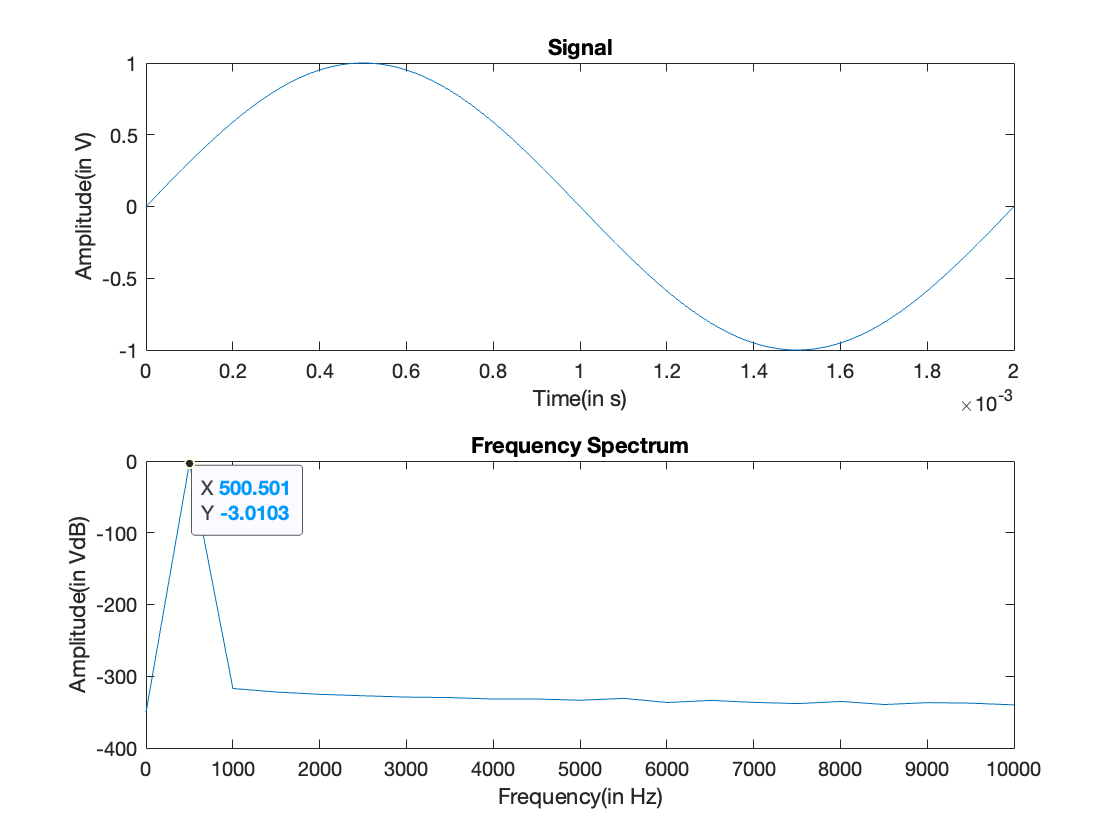
\includegraphics[width=0.75\linewidth]{images/evaluation_problem2.png}
              \caption{FFT of Single Tone sinusoidal wave}
              \label{fig:fft_single_tone}
          \end{figure}
          The calculated spectra seems to be in-line with what is seen in the oscilloscope, although there are no minor disturbances which are caused by the leakage of the windowing function used by the oscilloscope.
          The code used to generate the FFT is shown in the appendix.

    \item The MATLAB calculation of the FFT of the signal is shown in the figure below. In order to get a 0dB spectral peak, the voltage must be $sqrt(2)$, which is 1.414V or $2.82V_{pp}$.
          \begin{figure}[H]
              \centering
              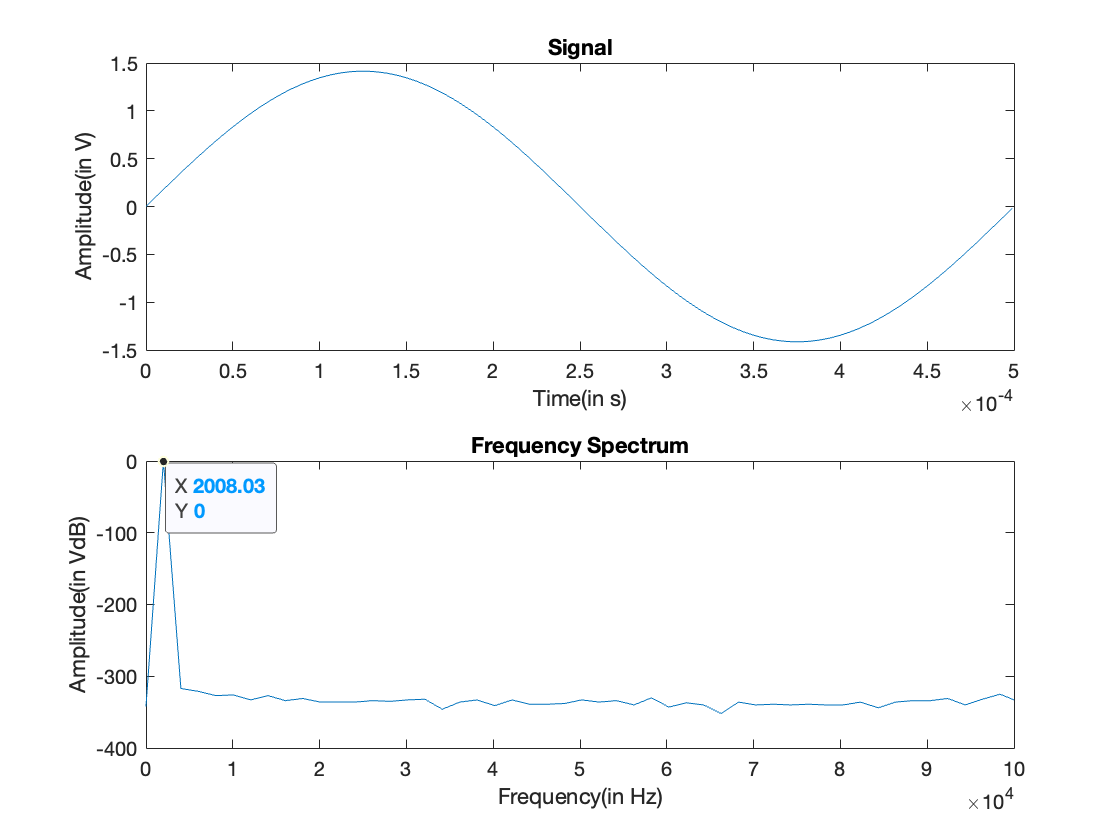
\includegraphics[width=0.75\linewidth]{images/evaluation_problem3.png}
              \caption{FFT showing 0dB spectral peak}
              \label{fig:fft_0dB_spectral_peak}
          \end{figure}
          The code used to generate the FFT is shown in the appendix.
    \item The results are in line with what is observed in the oscilloscope. The oscilloscope shows a -148mdB spectral peak when the voltage is $2.7V_{pp}$, which is close to the theoretical value of 0dB at $2.82V_{pp}$, the reason it is not exactly 0dB is because of the resolution of the oscilloscope.
\end{enumerate}

\section{Problem 2: FFT of a Square Wave}
\begin{enumerate}
    \item When the frequency scale is expanded to measure the frequency components of the signal, the bandwidth will decrease. The higher the bandwidth, the lower the resolution of the oscilloscope.
    \item In the 20\% duty cycle, it is observed that the signal can no longer be characterized by simply odd and even harmonics. Furthermore, every fifth harmonic has a significantly lower amplitude.
\end{enumerate}

\section{Problem 3: FFT of a multiple-tone signal}
\begin{enumerate}
    \item It is observed that when adding two signals together(a 1000KHz and 10,000KHz signal), the FFT of the signal is the sum of the FFT of the two signals. This is because the FFT is a linear operation, and we see the same behaviour in the oscilloscope, where it is observed that there are spikes at 1000KHz and 9900KHz, and knowing that both signals are sinusoids, it can be concluded that the resulting FFT is the sum of the FFT of the two signals.
\end{enumerate}